\subsubsection[Definition]{Definition}
\begin{minipage}{0.4\textwidth}
	\begin{framed}
		\centering
		$(f * g)(t):=\int_{-\infty}^{\infty} f(u) \cdot g(t-u) d u$
	\end{framed}
\end{minipage}\\
%
\begin{figure}[h]
	\centering
	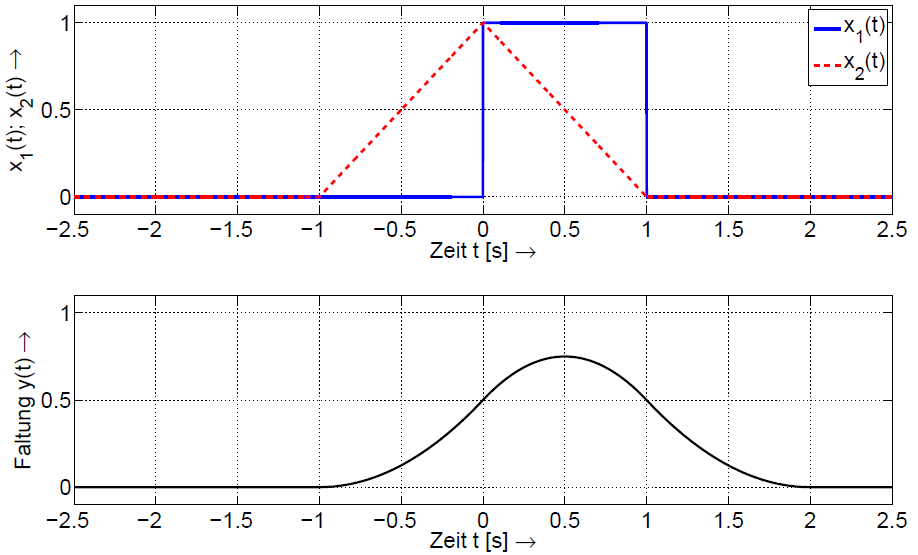
\includegraphics[width=0.8\textwidth]{pics/IntegralTransformation/Faltung.png}
	\caption{Quelle: Skript SigSys}
\end{figure}
%
\subsubsection[Rechenregeln]{Rechenregeln}
	\begin{minipage}{0.33\textwidth}
		\textbf{Kommutativität}\\
		$f *(g * h)=(f * g) * h$
	\end{minipage}
%
	\begin{minipage}{0.33\textwidth}
		\textbf{Assoziativität}\\
		$f *(g * h)=(f * g) * h$
	\end{minipage}
%
	\begin{minipage}{0.33\textwidth}
		\textbf{Distributivität}\\
		$f *(g+h)=(f * g)+(f * h)$
	\end{minipage}\\
%
\subsubsection[Faltung mit der $\delta$-Funktion]{Faltung mit der $\delta$-Funktion}
\begin{minipage}{0.5\textwidth}
	$f(t) * \delta\left(t-t_{0}\right)=f\left(t-t_{0}\right)$
\end{minipage}\\
%
